We compare the behaviour of applying the same GPTS Learner of the previous experiment (this time in presence of all the phases) with the performance of the SW GPTS Learner.
\\The experiment shows that the standard GPTS performs better in the first and the second phase of the year.  The better performance in the first phase is due to the fact that while the SW-GPTS always keep at maximum 1 month of memory, the basic GPTS keeps collecting samples. 
\\While comparing the second phase we can see that the performance of convergence of the two learners is quite the same. The standard GPTS does not suffer too much the fact that the first phase has ended because it is only a transition bethween a high interest phase and a low interest phase and therefore the budget allocation does not change too much among the classes of users.
\\The presence of a competitor change a lot into the budget allocation. It is not enougth to allocate the budget with respect of the average client of the brand because our company now need to invest more on a class to gain the same results on it, but the budget is limited. A choice is then needed in the third and the fourth phases and this explains the different behaviour. 
\\After about one month of exploration the SW-GPTS is able to converge in this new phase while we see that the basic GPTS will not converge anymore from now on: the sample collected in the preceding months weights too much on the choice of the budget allocation.
\\The regret chart that resulted from this experiment and the reward collected for each day are reported in the below figures.\\
\makebox[\textwidth][c]{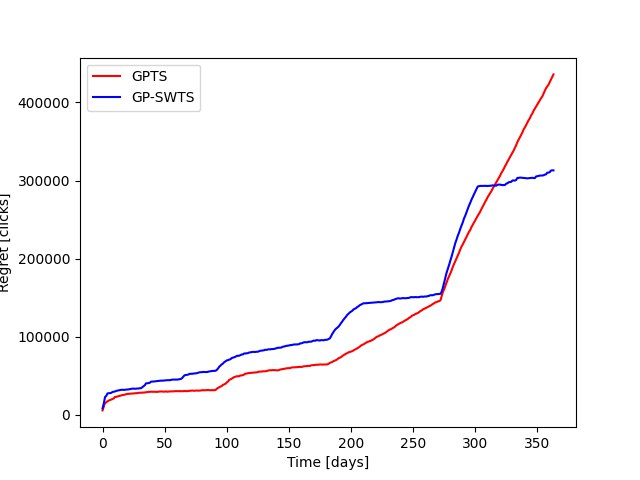
\includegraphics[width=0.85\textwidth]{../curves/results/swgpts-tmp-regret}}
\newpage
\makebox[\textwidth][c]{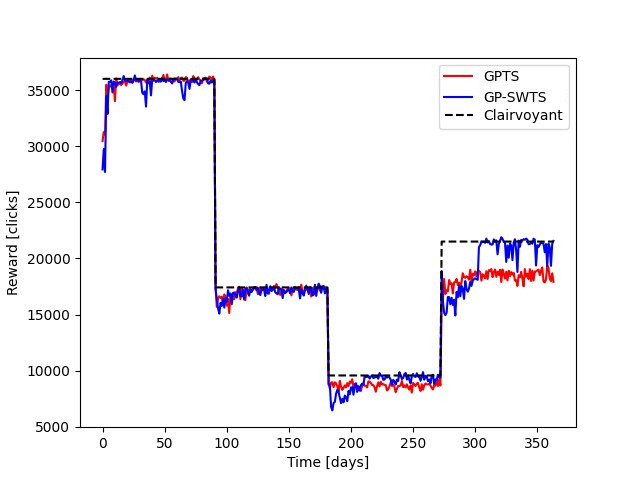
\includegraphics[width=0.85\textwidth]{../curves/results/swgpts-tmp-reward}}